% Generic TikZ sample used by the tests. Regenerate the SVG with:
%   python3 tikz2drawio.py tests/fixtures/tikz_sample.tex --keep-svg -o tests/fixtures
\documentclass[tikz,border=3pt]{standalone}
\usepackage{tikz}
\usetikzlibrary{arrows.meta,patterns}
\begin{document}
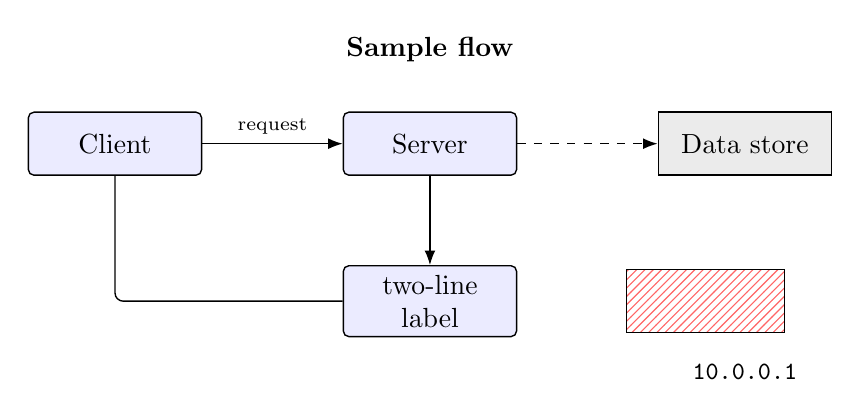
\begin{tikzpicture}[>=Latex, line width=0.5pt,
  box/.style={draw, rounded corners=2pt, minimum width=22mm, minimum height=8mm, fill=blue!8},
  plain/.style={draw, minimum width=22mm, minimum height=8mm, fill=black!8}]
  \node[box] (a) at (0,0) {Client};
  \node[box] (b) at (4,0) {Server};
  \node[plain] (c) at (8,0) {Data store};
  \node[box, align=center] (d) at (4,-2) {two-line\\label};
  \draw[->] (a) -- (b) node[midway, above, font=\scriptsize] {request};
  \draw[->, dashed] (b) -- (c);
  \draw[<-] (d) -- (b);
  \draw[rounded corners=3pt] (a.south) |- (d.west);
  \draw[pattern=north east lines, pattern color=red!60] (6.5,-2.4) rectangle (8.5,-1.6);
  \node[font=\bfseries] at (4,1.2) {Sample flow};
  \node[font=\ttfamily\small] at (8,-2.9) {10.0.0.1};
\end{tikzpicture}
\end{document}
